\section{How to Test the Rational Programmer} 
\label{sec:rational}

Code migration is the raison d'\^etre of Typed Racket, which is why the community
uses ``migratory typing'' instead of gradual typing. Roughly speaking a
programmer uses a gradually typed language to incrementally add types to a code
base. From this perspective, a code base consists of some number of components,
say modules, and a programmer converts a component at a time from its untyped
state to a typed one. 

Based on this idea, migratory paths offer a concise setting for
evaluating the effectiveness of a rational programmer for dealing with the
interesting debugging scenarios  from section ~\ref{sec:mutate}.
If we group debugging scenarios by mutation, then we obtain a set 
of programs that all contain the same mistake but differ in their type
annotations.  In the setting of migratory typing,\footnote{The method can be adapted to
so-called true gradual typing systems~\cite{svcb-snapl-2015} in a
straightforward manner.} each scenario differs from another in which
components are typed. Formally, a program $\system$ is a set of
components $\set{\component}$, and a scenario $\conf$ is the typed subset of
$\set{\component}$ . Hence, the scenarios of $\system$ are ordered by the
subset relation and, naturally,  form a lattice $\lattice{\system}$ with
$2^{\size{\system}}$ elements, like
the one introduced by ~\citet{tfgnvf-popl-2016} for performance
evaluations. The bottom scenario of
$\lattice{\system}$ is always $\emptyset$ and the top one is $\system$
itself. In between are all the mix-typed scenarios.


With these definitions, the actions of the rational programmer map to an
ascending chain---dubbed a \emph{trail}---in $\lattice{\system}$.  The
starting scenario $\conf_0$ of a trail---also referred to as the
\emph{root} (of the trail)---is the initial debugging scenario.  Herein we
consider only roots that are interesting debugging scenarios as described
in~\ref{sec:mutate} --- we expand on this point further on.  Intuitively,
starting from such a root, the rational programmer  steps along a trail,
and at each step, reduces the current scenario to an ``easier'' next
scenario to debug.  The easiest scenarios are those that the type checker
rejects outright, because a type error pinpoints an impedance mismatch
between the broken code of one component and its typed interface to
others. At this point, the programmer has identified the broken component.
If the scenario type-checks, the programmers runs the program until it
raises a run time error.  The rational programmer uses the error's blame
assignment\footnote{Blame can result either directly from a run time type
check or, in the absence of blame, from an exception that we track back to
the component that causes it with the help of the stack trace.} to decide
which component(s) to equip with types. This choice constructs scenario
$\conf_{i+1}$ from $\conf_{i}$ and implies the creation of trail.  

% The successor of a scenario on a trail has more typed component;
% formally, configuration $\conf_{i+1}$ on the trail differs from its
% predecessor $\conf_{i}$ in that more components are typed.

The next three subsections specialize the trail-scenario idea to the
various semantics of gradual typing. Once this machinery is in place,
we use the fourth subsection to state the precise experimental
research questions that correspond to the high-level question on the
first page and to explain our experimental process. The final
subsection extends the development with a discussion of programmer effort. 


%% -----------------------------------------------------------------------------
\subsection{Modes of the Natural Rational Programmer} \label{sub:natural}

The Natural semantics assigns blame to exactly one boundary.  A blame assignment
has the following specific meaning: the typed component may make incorrect type
assumptions about the untyped component in its interface, or the correct
interface exposes a bug in the untyped component. Our setup rules out the first
alternative (but see section~\ref{sec:conclusion}), and therefore the rational
programmer extends the trail to a scenario that swaps out the untyped component
for its typed counterpart.

We can turn this description into a formal definition of the trail. 
\begin{quote}
\it A \emph{Natural blame trail} is a sequence of scenarios $\conf_0,...\conf_n$ of
a program $\system$ such that for all $0 \leq i \leq n - 1$, $\conf_i \subset
\conf_{i+1}$ and $\conf_{i+1} \setminus \conf_i =\{\blame{\system, \conf_i}\}$ where
$\blame{\system, \conf}$ denotes the component that $\conf$ blames.
\end{quote}

When the buggy untyped component of a program is replaced by the typed counterpart,
the type checker fails if this component causes the impedance mismatch. Hence, a
trail that ends at an ill-typed scenarios successfully pinpoints the location of
bugs. 
\begin{quote}
\it A Natural blame trail $\conf_0,...\conf_n$ in a lattice $\lattice{\system}$ is
\emph{successful} iff its last scenario $\conf_n$ does not type check.  A Natural
blame trail $\conf_0,..,\conf_n$ in a lattice $\lattice{\system}$ is \emph{failing}
iff $\conf_n$ type checks and the trail cannot be extended further.
\end{quote}
That is, failing Natural blame trails are those that have not reached a scenario that
reveals the bug at compile time and their last scenario does not blame an untyped component. Thus
the rational programmer gets no hints from the gradual type system on how to
continue the search for the bug.

While a successful Natural blame trail indicates that it 
pays off to heed blame assignments during debugging the trail's root, it does not answer whether
blame is a critical piece of the rational programmer's process.  For instance,
typing the top of stack trace of a failed run time type check, dubbed the
location of the exception, might be as useful as typing the blamed one.

To account for this situation, we devise a new mode of the Natural rational
programmer that follows a migration process based on exceptions:
\begin{quote}
\it A Natural exception trail is a sequence of scenarios $\conf_0,...\conf_n$ of a
program $\system$ such that for all $0 \leq i \leq n - 1$, $\conf_i \subset
\conf_{i+1}$ and $\conf_{i+1} \setminus \conf_i = \{\exception{\system, \conf_i}\}$
where $\exception{\system, \conf}$ denotes the location of the exception of $\conf$.
\end{quote}

Putting the two modes together, we can now compare the usefulness of blame 
and mere exceptions for debugging a scenario in the context of Natural semantics.
\begin{quote}
\it 
  Given a program $\system$ and a root $\conf_0$ in $\lattice{\system}$,
  Natural blame is \emph{more useful} than Natural exceptions for
  debugging $\conf_0$ iff 
  the Natural blame trail 
  that starts at $\conf_0$ is successful while the Natural exception trail that
  starts at $\conf_0$ is failing.
\end{quote}

%% -----------------------------------------------------------------------------
\subsection{Modes of the Transient Rational Programmer} \label{sub:transient}

The transient semantics assigns blame to a set of components. In this setting, a
blame assignment has the following meaning: the witness value to the impedance
mismatch may have crossed the boundaries between elements in the set, and each crossing
checked the value's type in a shallow manner. 

This ambiguity in Transient blame raises the question of how the rational programmer
should react when the language produces a blame set. Our answer is that the rational
programmer has at least two reasonable options. The first one is to select the component that is added
to the blame set first and assign types to only that one---after all, if
fully checked, the types of
this first component should be able to detect an impedance mismatch earlier in the
evaluation of a program than the later ones. The second option is to
select the component that is added to the blame set last, effectively
interpreting the blame set as a boundary-aware stack. 

These two modes of rationalizing give rise to two different notions of trail.
\begin{quote}
\it A \emph{Transient-first blame trail} is a sequence of scenarios
$\conf_0,...\conf_n$ of $\system$ where for all $0 \leq i \leq n - 1$,
$\conf_i \subset \conf_{i+1}$ and $\conf_{i+1} \setminus \conf_i =
\first{\mblame{\system, \conf_i}}$ where $\first{\mblame{\system, \conf}}$ is the
first component Transient adds to the blame set for $\conf$.
\end{quote}

and 

\begin{quote}
\it A \emph{Transient-last blame trail} is a sequence of scenarios
$\conf_0,...\conf_n$ of $\system$ where for all $0 \leq i \leq n - 1$,
$\conf_i \subset \conf_{i+1}$ and $\conf_{i+1} \setminus \conf_i =
  \last{\mblame{\system, \conf_i}}$ where $\last{\mblame{\system, \conf}}$ is the
last component Transient adds to the blame set for $\conf$.
\end{quote}

The definition of \emph{Transient exception trails} 
is analogous to that for Natural and, same as for Natural, we use it to  
specify when  
Transient-first and Transient-last blame are more useful than 
Transient exceptions for debugging a scenario.  


%% -----------------------------------------------------------------------------
\subsection{Modes of the Erasure Rational Programmer} \label{sub:erasure}

 Since gradually typed languages with Erasure semantics do not come with
 blame assignment, a rational programmer can only hope that the underlying
 safety checks and their exceptions are helpful.  Thus, the Erasure 
 rational programmer has a single mode, the Erasure exception mode, and
 its definition and the accompanying notion of usefulness follow that for
 Natural.

%% -----------------------------------------------------------------------------
\subsection{Experimental Process.}
\label{subsec:experiment}


Trails and their properties give us the tools for a rigorous examination
of blame for Natural, Transient and Erasure Typed Racket in the setting of the 
mutants from section~\ref{sec:mutate}. In line with the discussion so far, 
our experimental process collects data to answer three initial questions
for our interesting debugging scenarios:
\begin{itemize}
\item[$Q_1$] Is blame useful in the context of Natural?

\item[$Q_2$] Is first blame useful in the context of Transient?

\item[$Q_3$] Is last blame useful in the context of Transient?

\end{itemize}

Furthermore, our experiment can compare the relative usefulness of blame
between any two of the three semantics. 
\begin{itemize}
\item[$Q_*$] Is blame for X more useful than blame for Y? (Where X and Y are any of Natural, Transient, or Erasure)
\end{itemize}


Table~\ref{fig:experiment-outline} summarizes how each question relates to
different kinds of trails/modes of the rational programmer. For example, experimental
question $Q_1$ asks whether blame is valuable for Natural and our experiment
uses the Natural blame and exception trails to answer it.

\begin{figure}[ht]
\center
{\begin{tabular}{l|c|c|c}
%% ---------------------------------------------------------------------------------------------------------------
                        & {\bf Natural}  & {\bf Transient} &  {\bf Erasure} \\ \hline 
%% ---------------------------------------------------------------------------------------------------------------
{\bf Blame}             &  $Q_1/Q_*$    &                  &                \\
{\bf First blame}       &               &     $Q_2/Q_*$    &                 \\
{\bf Last blame}        &               &     $Q_3/Q_*$    &                 \\
{\bf Exceptions}        &      $Q_1$    &     $Q_2/Q_3$    &      $Q_*$      \\
\end{tabular}}
  \caption{ Experimental questions and rational programmer modes.}
  \label{fig:experiment-outline}
\end{figure}

%% -----------------------------------------------------------------------------

In detail we answer $Q_1$  by comparing the success of the 
Natural blame and Natural exception trails for all interesting 
debugging scenarios from section~\ref{sec:mutate}.
  The first step is to construct each
mutant's scenario lattice and identify their interesting debugging
scenarios.
Our test
bed extends the trails that start from such roots according to the Natural-blame programmer.  If no scenarios
can be added to the trail, we check if
the last scenario of the trail type-checks or not. If it does, we record that the Natural-blame
trail is successful, and otherwise that fails. We repeat the process for the
same roots again but for the other mode, Natural exceptions.
 Figure~\ref{fig:process}
summarizes this
experimental process for one mode of the rational programmer and connects
it with the mutations from section~\ref{sec:mutate}.
After completing the experiment, we calculate the
success/failure results of the trails to determine for each root whether Natural blame
is more useful than Natural exceptions. We
obtain a positive answer for
$Q_1$ when a root exists where the above is true since it is evidence that
there is at least one interesting scenario that the rational programmer
manages to debug because of blame. 
The process is analogous for $Q_2$ and $Q_3$, employing the respective
modes of the rational programmer.

For $Q_*$, the process is a bit more
involved. At a first level we proceed in a similar
manner except that we use two modes 
of the rational programmer from different semantics.
However, answering this question requires us to compare the percentage of scenarios
where one mode is more useful than the other and the inverse.
For instance, to
decide whether blame for Natural is more useful than first blame for Transient, 
we compare the percentage of interesting scenarios where 
Natural blame is more successful than Transient first blame 
with the percentage of interesting scenarios where Transient first blame 
is more successful than Natural blame. 
Finally we repeat these steps one more time to compare Natural blame and Transient last blame
and get a complete picture of the comparative usefulness of blame
in the two semantics.

\begin{figure}
  \centering
  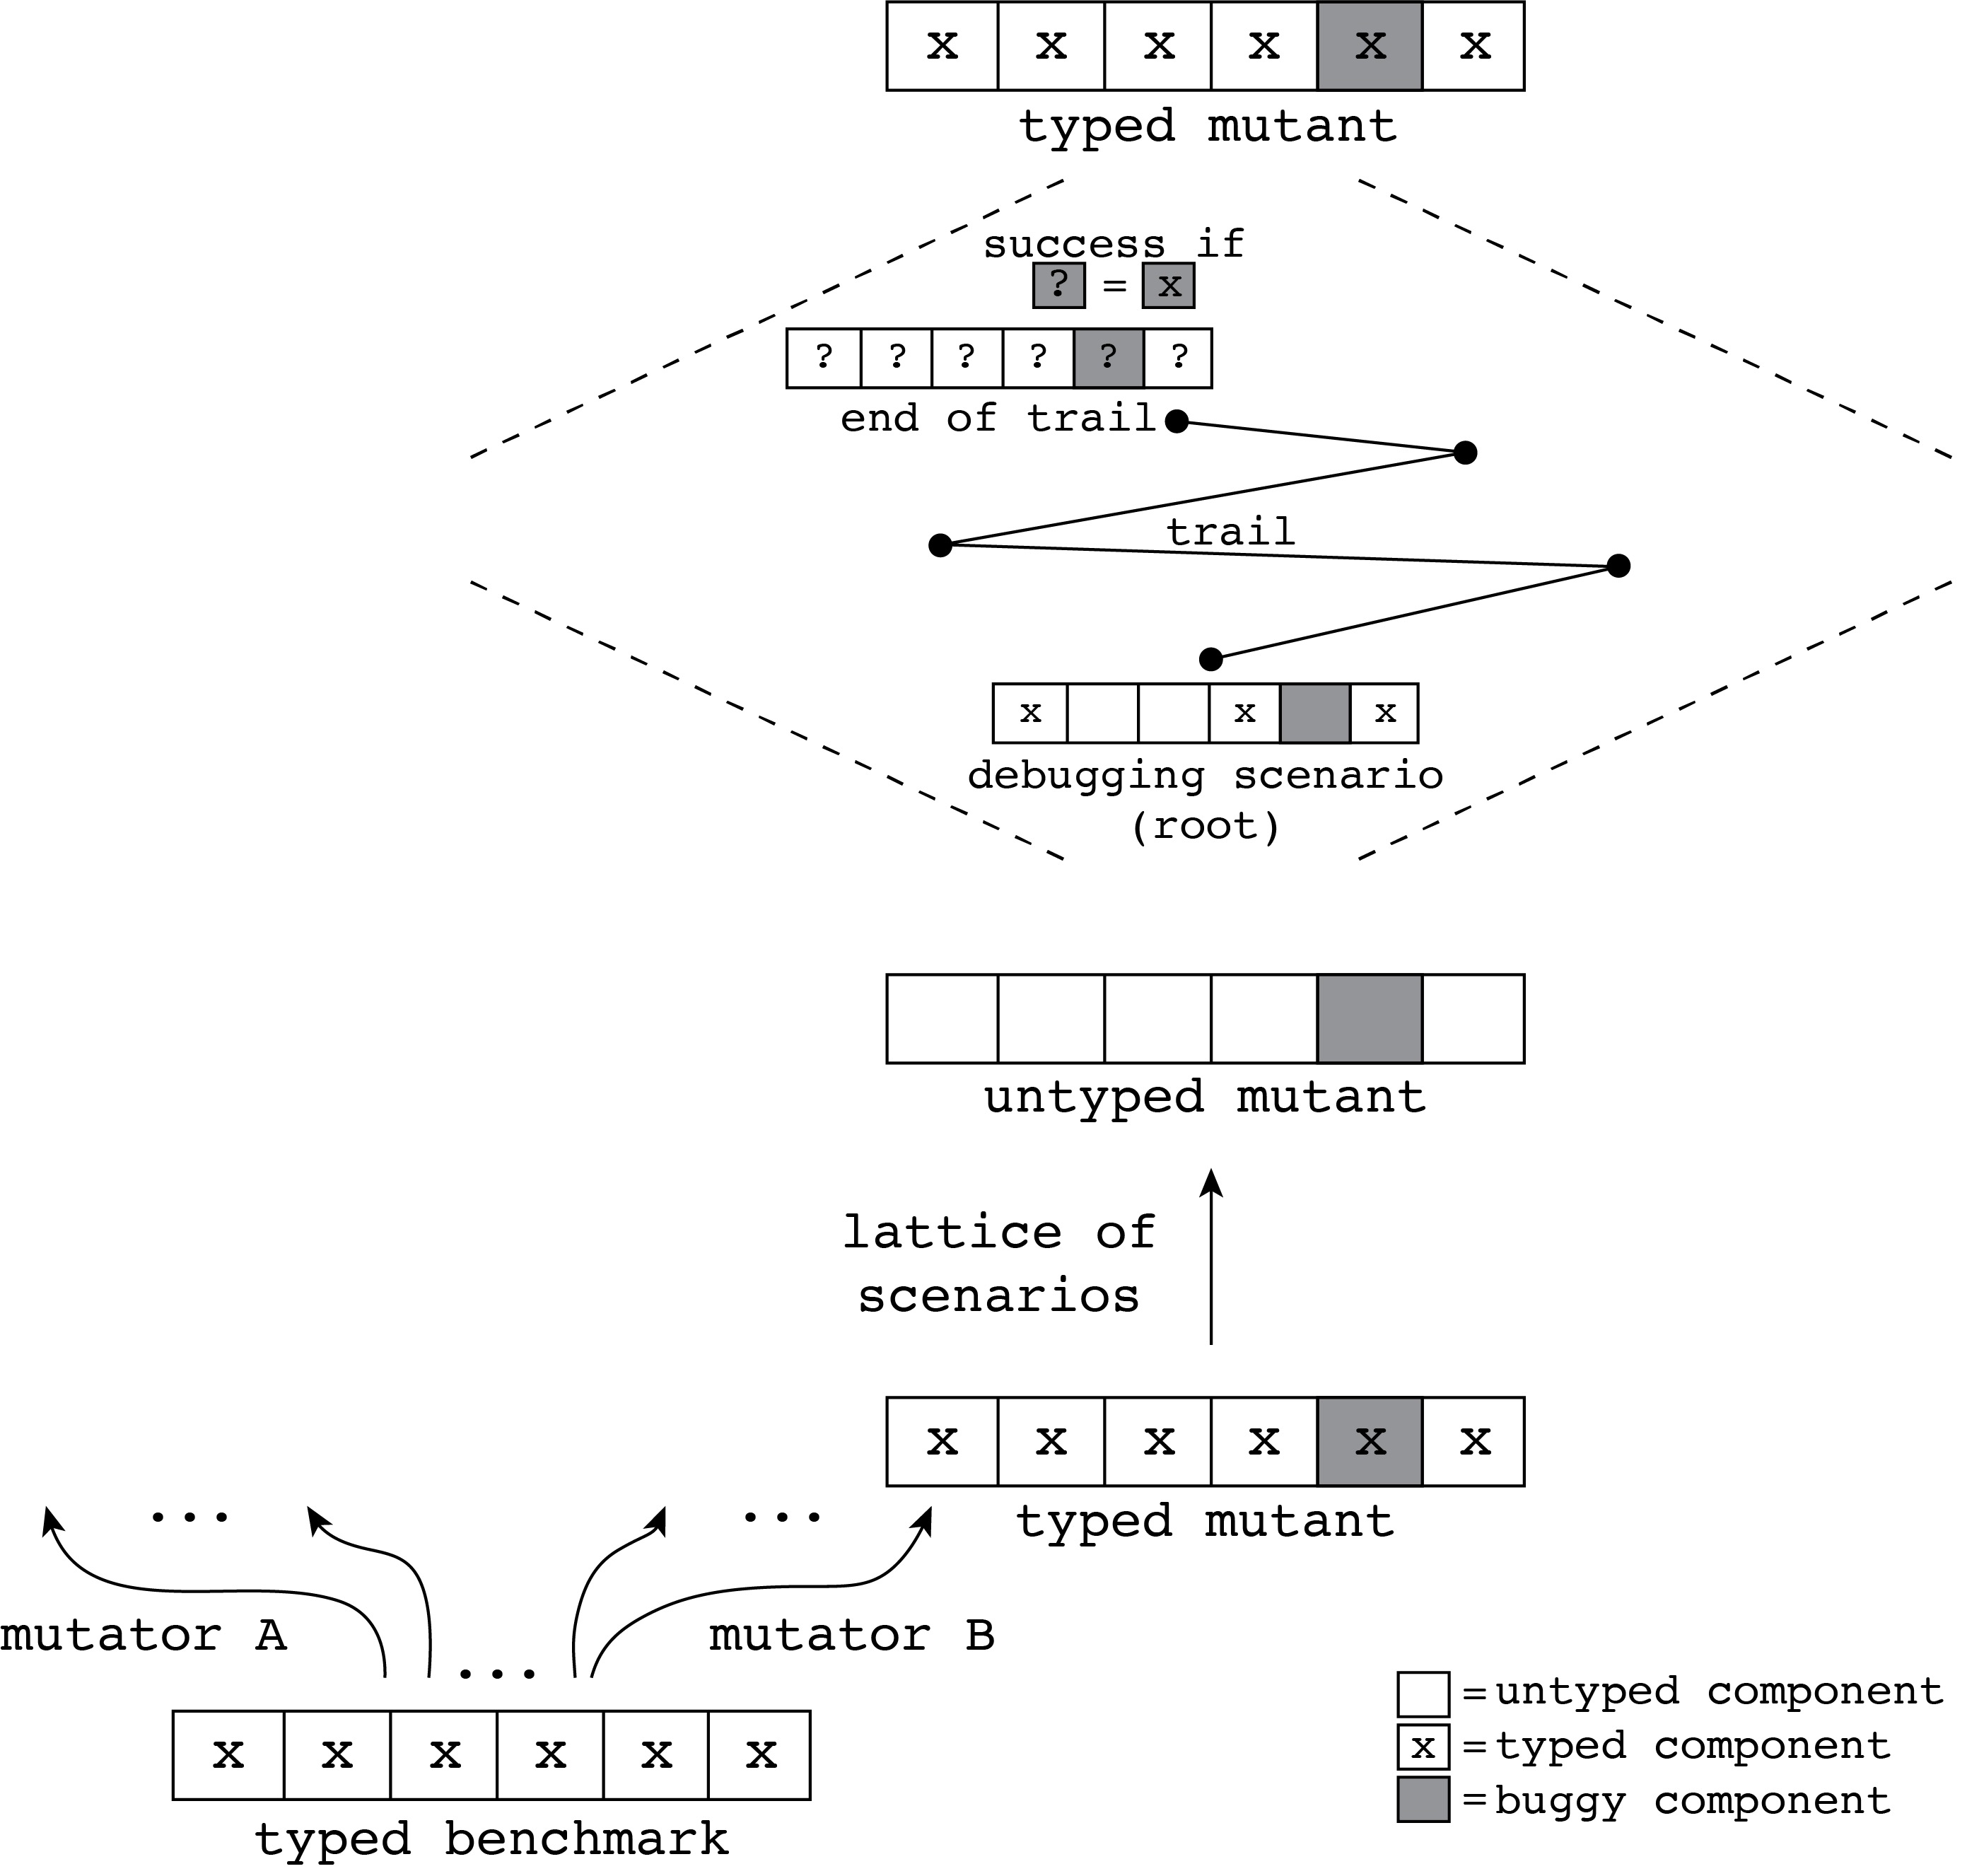
\includegraphics[scale=0.36]{./Images/process}
  \caption{The experimental process for one mode of the rational
  programmer}
  \label{fig:process}
\end{figure}


\subsection{Programmer Effort}
\label{subsec:effort}

In addition to successful and failure information for the various trails,  
our experiment  records the number of components a rational programmer 
has to type along each trail ($\lvert \conf_n \setminus \conf_0
\rvert$). We use this number as the metric for the effort 
of the rational programmer to debug an interesting scenario.  

A comparison of the effort of different modes of the rational programmer
can help shed some further light to the effectiveness of the
three gradual typing systems. For example, consider one debugging scenario.  
If, for instance, both  Natural blame and Transient first
blame trails are successful, the two modes of the 
rational programmer can compete to see which one
debugs the interesting scenario with less effort. In
general, if the effort distribution for a mode of the rational programmer
has a shorter tail and more
volume around smaller values compared to the effort distribution of another
mode, then this is evidence that the first mode is the more effective of the two.  

Finally, effort allows us to test whether the observed effectiveness 
of the rational programmer is an artifact of pure chance or not.
That is, we can compare the effort distribution for a mode of the
rational programmer with another mode that ignores error information entirely
and instead selects which component to type next randomly. 
Of course, since each mutant has a finite number of components, 
such random mode trails are always successful. At the same time though,
the Natural, Transient, and Erasure random modes exhibit a normal effort
distribution across scenarios that should be distinct from the effort distribution for all other modes of
the rational programmer if the effectiveness of the modes are not
coincidental.




